\chapter{Нечёткие множества}

%fuz: label prefix
Нечеткие множества нашли широкое применение в области искусственного интеллекта и управления. Действительно, в этих областях весьма часто требуется задавать некоторые логические правила (отражающие знания или определяющие поведение объекта управления). Элементами этих правил могут являться весьма <<нечёткие>> понятия\ldots Допустим, что <<умная>> компьютерная система управления теплицей руководствуется следующими правилами, снимая показания температуры \verb"t" с датчика над кустом томатов:
\begin{verbatim}
Если t холодно,    то включить_отопитель,выключить_охладитель;
Если t оптимально, то ничего_не_делать;
Если t жарко,      то выключить_отопитель,включить_охладитель;
\end{verbatim}

В данных правилах используются следующие качественные описания температуры: \verb"холодно", \verb"оптимально", \verb"жарко". И, пожалуй, эти правила управления нас устроят, если мы на место томатов посадим пальму. Но пальму они не устроят, потому что то, что для томатов \verb"оптимально" (не говоря о \verb"холодно"), то пальме --- смерть! Очевидно, что под \verb"холодно", \verb"оптимально", \verb"жарко" понимаются некоторые множества --- диапазоны температур. Пойдя навстречу пальме, попытаемся изменить эти множества. Но мы столкнемся с некоторыми трудностями: 
\begin{itemize}
    \item[]\emph{Вы:} 22 градуса по цельсию --- для Вас \verb"оптимально"?
    \item[]\emph{Пальма:} Близко к оптимальному, да\ldots Но уже чуток холодновато\ldots 
    \item[]\emph{Вы:} Значит \verb"холодно"?
    \item[]\emph{Пальма:} Нет, нет, не холодно, ну, пожалуй чуток\ldots 
    \item[]\emph{Вы:} Значит все же \verb"оптимально"?
    \item[]\emph{Пальма:} Процентов на 90\ldots см. рис. \ref{fig:fuz:fuzzyTemperature}!!!
    \item[]\emph{Вы:} \ldots
\end{itemize}

Вот тут и пригодятся нечеткие множества. Понятие нечетких множеств было введено Л.~Заде в 1965 году. Изложение  математических основ можно найти, например, в \cite{bib:gorbatovs:discrmath} или в прикладном контексте\footnote{Данная книга посвящена нейронным сетям --- важной области искусственного интеллекта} в \cite{bib:osovsky:neyro}. Краткая теория приведена ниже.


\section{Основные определения}

Множество $A$, являющееся подмножеством некоторого универсального множества $U$, можно задать с помощью \emph{характеристической функции} (\emph{функции принадлежности}), определенной следующим образом для каждого $x\in U$:
\[
    \label{eq:fuz:charFhard}
    \mu_A(x)=
    \begin{cases}
        1,&\text{если $x\in A$},\\
        0 &\text{в противном случае.}
    \end{cases}
\]

Итак, если для некоторого $x\in U$ функция $\mu_A(x)=1$, то $x$ принадлежит множеству $A$, если $\mu_A(x)=0$, то $x$ множеству $A$ не принадлежит. Для \emph{нечеткого} множества $A$ характерно то, что $\mu_A(x)$ принимает значение из отрезка $[0,1]$. Нечёткое множество $A\subseteq U$ определяется так:
\[
    A=\{x/\mu_A(x)|x\in U\}.
\]

Конкретное значение $\mu_A(x)$ называется \emph{коэффициентом принадлежности} элемента $x$ множеству $A$. То есть $\mu_A(x)$ определяет степень принадлежности $x$ множеству $A$. Если $\mu_A(x)>\mu_A(y)$, то элемент $x$ принадлежит множеству $A$ в большей степени, чем $y$.
\begin{exampl}
    Нечеткое множество <<большой>> на универсуме <<животные>> для попугая выглядит так: 
    \[
        \begin{split}
            \text{большой}=\{
                \text{попугай}/1,\text{жираф}/0.98,\text{слон}/0.9,\\
                \text{удав}/0.5,\text{зебра}/0.4,\text{гиена}/0.3,\\
                \text{мартышка}/0.2,\text{клоп}/0.01,\text{кит}/0\}.
        \end{split}
    \]
    Как видно, коэффициенты $\mu_{\text{большой}}(x)$ сильно зависят от опыта <<эксперта>>: например, можно сказать, что попугай ни разу в жизни не видел кита. В этом отличие коэффициента принадлежности от, например, вероятности, с которой его часто путают.
    \qed
\end{exampl}

Когда универсальное множество $U$ бесконечно(счетно или континуально), то для того, чтобы задать $\mu_A(x)$ часто используют следующего вида аналитические функции (см. рис. \ref{fig:fuz:fuzzyTemperature}): 
\begin{itemize}
    \item сигмоидальные:
    \[
        \mu_A(x)=\frac{1}{1+\exp\left[-a(x-c)\right]},\mu_A(x)=\frac{x-c}{2(a+|x-c|)}+\frac{1}{2};
    \]
    
    \item гауссовские:
    \[
        \mu_A(x)=\exp\left[-\left(\frac{x-c}{d}\right)^{2b}\right],
        \mu_A(x)=\frac{1}{1+\left(\frac{x-c}{d}\right)^{2b}};
    \]
\end{itemize}

иногда используют фрагменты линейных функций, определенных на соответствующих интервалах (см. например, рис. \ref{fig:fuz:fuzzyOperations}).

\begin{figure}
    \centering
    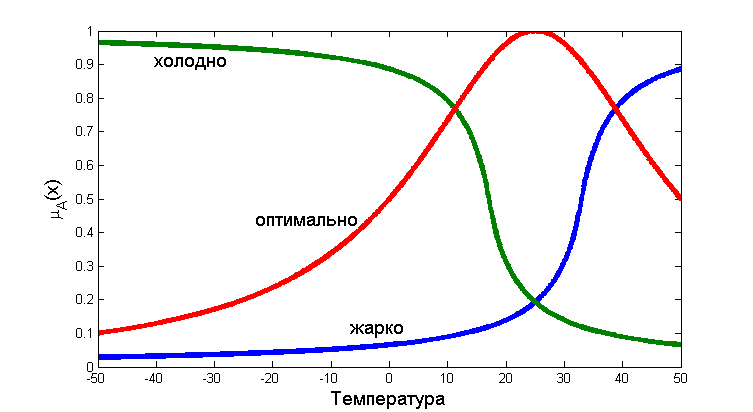
\includegraphics[width=0.8\textwidth]{fig/fuzzyTemperature}
    \caption{Аналитически заданные функции $\mu_A(x)$ для градаций температуры}
    \label{fig:fuz:fuzzyTemperature}
\end{figure} 


\section{Операции над нечеткими множествами}

Над нечеткими множествами $A,B$ выделяют следующие основные операции:
\begin{enumerate}
    \item Объединение $A\cup B$: $\mu_{A\cup B}(x)=\max[\mu_A(x),\mu_B(x)]$;
    \item Пересечение $A\cap B$: $\mu_{A\cap B}(x)=\min[\mu_A(x),\mu_B(x)]$
    \item Отрицание $\overline{A}$: $\mu_{\overline{A}}(x)=1-\mu_A(x)$;
    \item Вычитание $A\backslash B$: $\mu_{A\backslash B}(x)=\min[\mu_A(x), 1-\mu_B(x)]$;
    \item Концентрация $CON(A)$: $\mu_{CON(A)}(x)=[\mu_A(x)]^2$;
    \item Растяжение $DIL(A)$: $\mu_{DIL(A)}(x)=\sqrt{\mu_A(x)}$;
    \item Нормализация $NORM(A)$: $\mu_{NORM(A)}(x)=\frac{\mu_A(x)}{\sup\{\mu_A(y)|y\in U\}}$;
\end{enumerate}

Необходимо отметить, что в отличие от <<обычных>> множеств, одноименные операции не обладают теми же свойствами, в частности:
\begin{itemize}
    \item $A\cup\overline{A}\neq U$;
    \item $A\cap\overline{A}\neq\emptyset$.
\end{itemize}

$A\subseteq B$, если $\forall x\in U (\mu_A(x)\leq\mu_B(x))$. Для равенства: $A=B\Leftrightarrow (A\subseteq B)\land(B\subseteq A)$.

В нечеткой логике нечеткому множеству соответствует так называемая \emph{лингвистическая переменная}. И операции над нечеткими множествам соответствуют логическим связкам между лингвистическими переменными (см. рис. \ref{fig:fuz:fuzzyOperations}). Например, объединение соответствует связке <<ИЛИ>>, пересечение --- <<И>>, отрицание --- <<НЕ>>. Концентрация соответствует прилагательному <<ОЧЕНЬ>> перед лингвистической переменной, а растяжение --- прилагательным <<ПОЧТИ>>,<<ПРИМЕРНО>> (см. рис. \ref{fig:fuz:fuzzyConDil}).

\begin{figure}
    \centering
    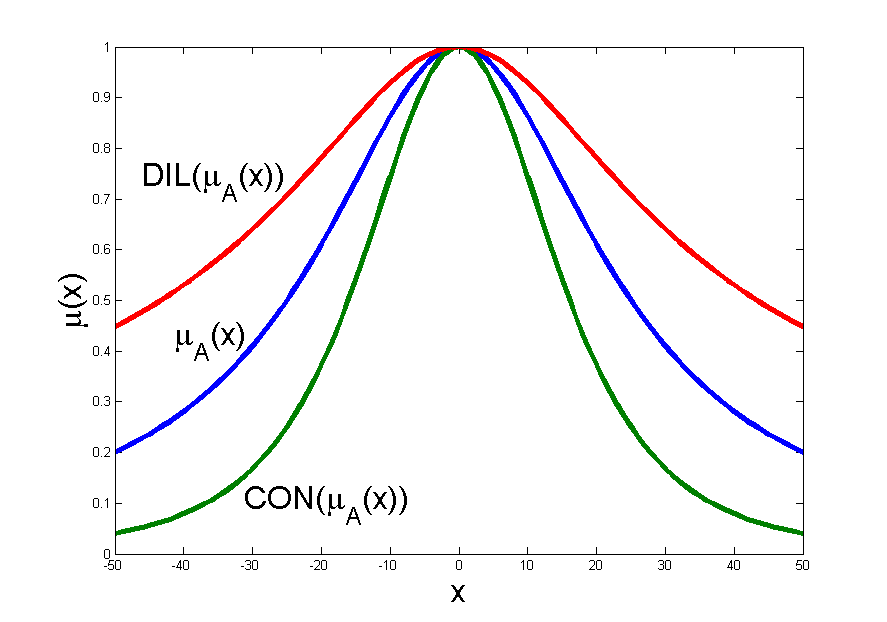
\includegraphics[width=0.8\textwidth]{fig/fuzzyConDil}
    \caption{Концентарция и растяжение нечёткого множества $A$}
    \label{fig:fuz:fuzzyConDil}
\end{figure} 


\begin{figure}
    \centering
    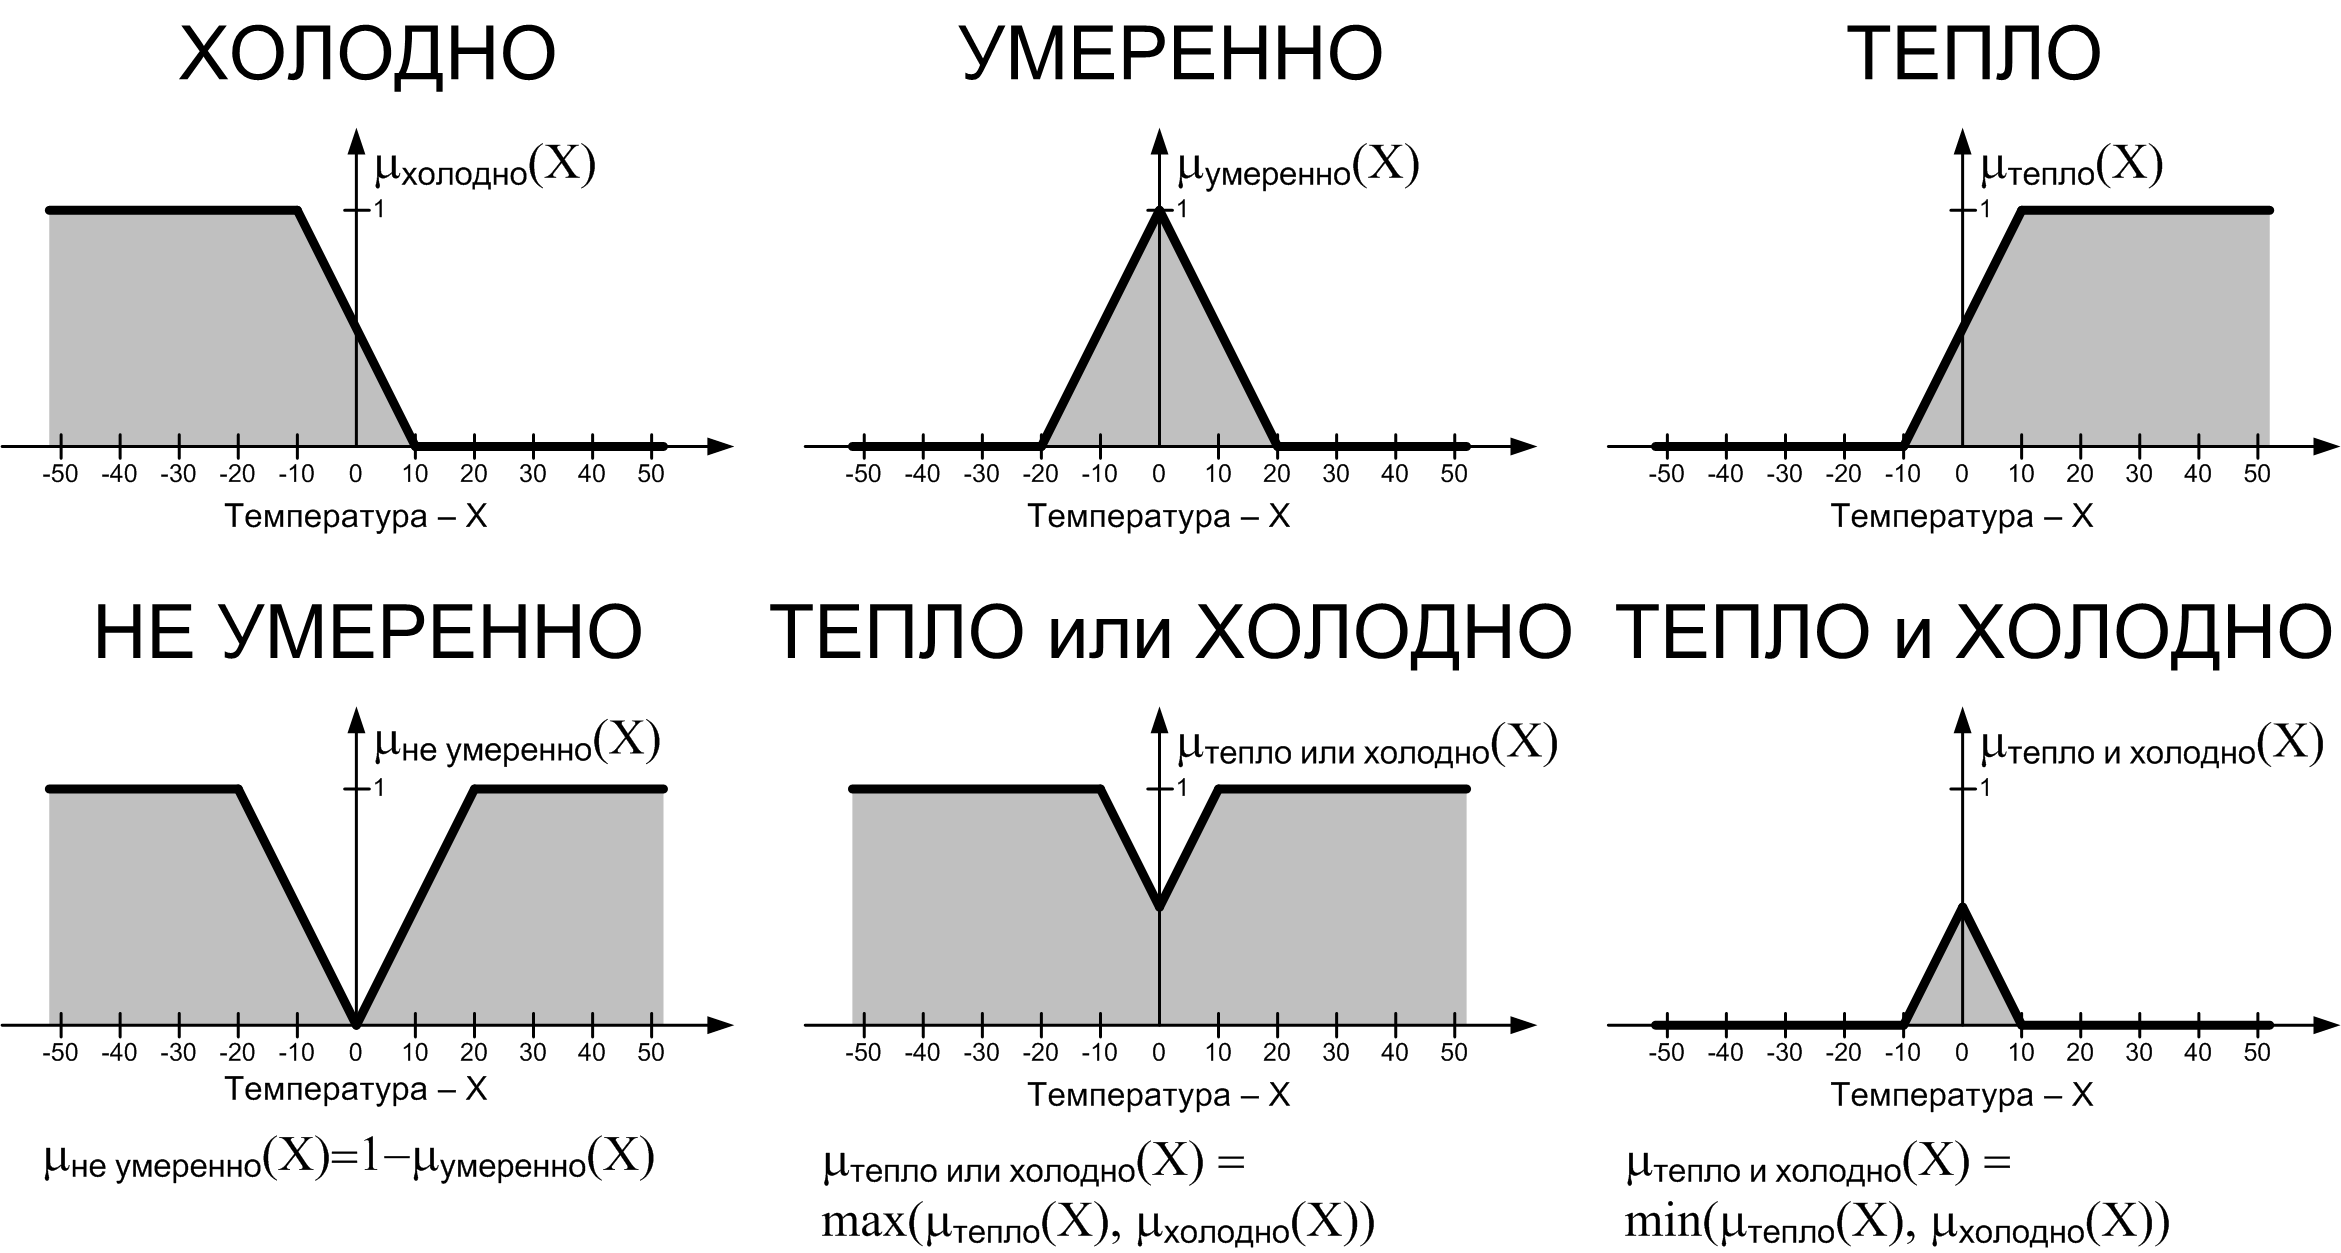
\includegraphics[width=0.9\textwidth]{fig/fuzzyOperations}
    \caption{Логические связки между лингвистическими переменными соответствуют операциям над нечеткими множествами}
    \label{fig:fuz:fuzzyOperations}
\end{figure} 

Видно, что бинарные операции основаны на функциях $\min$ и $\max$. В общем случае вместо $\min$ используют функцию $T:[0,1]\times[0,1]\to[0,1]$, которая называется \emph{$t$-нормой}, а вместо $\max$ используют функцию $S:[0,1]\times[0,1]\to[0,1]$, которая называется \emph{$t$-конормой}. $t$-норма обладает следующими свойствами:
\begin{enumerate}
    \item ограниченность: $T(0,0)=0,T(1,\mu)=\mu,T(\mu,1)=\mu$;
    \item монотонность: $T(\mu_1,\mu_2)\leq T(\mu_3,\mu_4)$, если $\mu_1\leq\mu_3, \mu_2\leq\mu_4$;
    \item коммутативность: $T(\mu_1,\mu_2)=T(\mu_2,\mu_2)$;
    \item ассоциативность: $T(\mu_1,T(\mu_2, \mu_3))=T(T(\mu_1,\mu_2),\mu_3)$;
\end{enumerate}

Примерами $t$-норм могут являться функции:
\begin{itemize}
    \item $T(\mu_1,\mu_2)=\min(\mu_1,\mu_2)$;
    \item $T(\mu_1,\mu_2)=\mu_1\cdot \mu_2$;
    \item $T(\mu_1,\mu_2)=\max[0,\mu_1+\mu_2-1]$.
\end{itemize}

$t$-конорма обладает следующими свойствами:
\begin{enumerate}
    \item ограниченность: $S(1,1)=1,S(0,\mu)=\mu,S(\mu,0)=\mu$;
    \item монотонность: $S(\mu_1,\mu_2)\geq S(\mu_3,\mu_4)$, если $\mu_1\geq\mu_3, \mu_2\geq\mu_4$;
    \item коммутативность: $S(\mu_1,\mu_2)=S(\mu_2,\mu_2)$;
    \item ассоциативность: $S(\mu_1,S(\mu_2, \mu_3))=S(S(\mu_1,\mu_2),\mu_3)$;
\end{enumerate}

Примерами $t$-конорм могут являться функции:
\begin{itemize}
    \item $S(\mu_1,\mu_2)=\max(\mu_1,\mu_2)$;
    \item $S(\mu_1,\mu_2)=\mu_1+\mu_2-\mu_1\cdot\mu_2$;
    \item $S(\mu_1,\mu_2)=\min[1,\mu_1+\mu_2]$.
\end{itemize}

Нечеткие множества лежат в основе нечеткой логики, рассмотрение которой выходит за рамки данного курса. Заинтересовавшимся практическим применением нечеких множеств можно рекомендовать \cite{bib:osovsky:neyro}.

\section*{Задания}
\addcontentsline{toc}{section}{Задания}

\begin{enumerate}
    
    \item Доказать, что $t$-конорма $T(\mu_1,\mu_2)=\mu_1+\mu_2-\mu_1\cdot\mu_2$ это функция $T:[0,1]\times[0,1]\to[0,1]$. Т.е. что $\rho_T=[0,1]$. Также доказать, что она ассоциативна.
    %a+b-ab = a(1-b)+b = a(1-b)+b-1+1 = a(1-b)-(1-b)+1 = 1-(1-a)(1-b)
    
    \item Докажите, что для нечеткого множества $A$ справедливо $A\subseteq DIL(A)$.
    
    \item Нечеткие множества на универсуме <<насекомое>> заданы в таблице \ref{table:fuz:insectos}. Найти нечеткое множество, соответствующее лингвистической переменной:
    \begin{enumerate}
        \item Опасно и не опасно
        \item Очень опасно
        \item Большое и не опасно
        \item Спутник и опасно
        \item Яркое и сильное
        \item (Яркое или большое) и не плодовитое
    \end{enumerate}

    Найдется ли среди представленных в таблице \ref{table:fuz:insectos} множество, являющееся подмножеством какого-либо другого множества.
    \begin{table}
        \centering
        \begin{tabular}{l||c|c|c|c|c|}
            Переменная&
                                \rotatebox{90}{Скорпион}&
                                        \rotatebox{90}{Пчела}&
                                                \rotatebox{90}{Шершень}&
                                                        \rotatebox{90}{Капустница}&
                                                                \rotatebox{90}{Муравей} \\
            \hline\hline
            Опасно(для человека)&0.5    &0.4    &0.5    &0.01   &0.1    \\ \hline
            Большое             &0.8    &0.2    &0.7    &0.6    &0.01   \\ \hline
            Яркое               &0.2    &0.1    &0.5    &0.5    &0.01   \\ \hline
            Сильное             &0.5    &0.3    &0.4    &0.01   &0.99   \\ \hline
            Плодовито           &0.1    &0.9    &0.1    &0.8    &0.9    \\ \hline
            Спутник(человека)   &0.1    &0.8    &0.2    &0.5    &0.1    \\ \hline
        \end{tabular}
        \caption{Лингвистические переменные на универсуме насекомых}
        \label{table:fuz:insectos}
    \end{table}

    \item Докажите справедлив ли закон дистрибутивности операций над нечеткими множествами $A\cap(B\cup C)=(A\cap B)\cup (A\cap C)$ и $A\cup(B\cap C)=(A\cup B)\cap (A\cup C)$, если в качестве пары ($t$-норма,$t$-конорма) выбрана пара:
    \begin{enumerate}
        \item $(\min,\max)$;
        \item $(\mu_1\cdot\mu_2,\mu_1+\mu_2-\mu_1\cdot\mu_2)$.
    \end{enumerate}
    
\end{enumerate}
